\documentclass[11pt,a4paper]{article}

\usepackage[T1]{fontenc}
\usepackage[utf8]{inputenc}
\usepackage[french]{babel}
\usepackage{lmodern}
\usepackage{microtype}
\usepackage[a4paper,margin=2.4cm,headheight=24pt]{geometry}
\usepackage{graphicx}
\usepackage{float}
\usepackage{booktabs}
\usepackage{array}
\usepackage{longtable}
\usepackage{tabularx}
\usepackage{enumitem}
\usepackage{xcolor}
\usepackage{setspace}
\usepackage{fancyhdr}
\usepackage{titlesec}
\usepackage{hyperref}
\usepackage{caption}
\usepackage{needspace}
\usepackage{tikz}
\usepackage{tcolorbox}

\hypersetup{
  colorlinks=true,
  linkcolor=blue!50!black,
  citecolor=blue!50!black,
  urlcolor=blue!60!black,
  pdftitle={Rapport Projet Django - Gestion de Stock},
  pdfauthor={AMLLAL Amine},
  pdfsubject={Rapport technique et fonctionnel}
}

\setstretch{1.15}
\setlength{\parskip}{0.45em}
\setlength{\parindent}{0pt}

\definecolor{mainblue}{HTML}{123B6D}
\definecolor{accent}{HTML}{E55C2B}
\definecolor{tealnote}{HTML}{0E7C7B}
\definecolor{lightgray}{HTML}{F3F5F7}
\definecolor{pagebg}{HTML}{FFFFFF}

\pagecolor{pagebg}
\color{black}

\titleformat{\section}
  {\Large\bfseries\color{mainblue}}
  {\thesection}{0.8em}{}
  [\vspace{0.2em}\color{accent}\titlerule]
\titleformat{\subsection}
  {\large\bfseries\color{tealnote}}
  {\thesubsection}{0.7em}{}
\titleformat{\subsubsection}
  {\normalsize\bfseries\color{mainblue}}
  {\thesubsubsection}{0.6em}{}

\pagestyle{fancy}
\fancyhf{}
\fancyhead[L]{\textcolor{mainblue}{\textbf{Gestion de Stock}}}
\fancyhead[R]{\textcolor{tealnote}{\textbf{AMLLAL Amine}}}
\fancyfoot[C]{\textcolor{accent}{\thepage}}
\renewcommand{\headrulewidth}{0.8pt}
\renewcommand{\footrulewidth}{0.4pt}
\renewcommand{\headrule}{\hbox to\headwidth{\color{mainblue}\leaders\hrule height \headrulewidth\hfill}}
\renewcommand{\footrule}{\hbox to\headwidth{\color{accent}\leaders\hrule height \footrulewidth\hfill}}

\begin{document}

\pagenumbering{gobble}

\begin{titlepage}
\thispagestyle{empty}
\begin{center}
\vspace*{1.2cm}

\begin{tikzpicture}
  \node[rounded corners=3pt, fill=mainblue!9, draw=mainblue, line width=0.6pt, inner xsep=14pt, inner ysep=6pt]
  {\textcolor{mainblue}{\textbf{Rapport Technique Professionnel}}};
\end{tikzpicture}

\vspace{1.4cm}

{\color{mainblue}\rule{0.9\textwidth}{1.5pt}}\par
\vspace{0.5cm}
{\Huge\bfseries Syst\`eme de Gestion de Stock\par}
\vspace{0.5cm}
{\Large Application Web Django}\par
\vspace{0.5cm}
{\color{mainblue}\rule{0.9\textwidth}{1.5pt}}\par

\vspace{2.2cm}

\begin{tabular}{>{\bfseries}p{4.2cm}p{9.5cm}}
R\'ealis\'e par : & AMLLAL Amine \\
Encadr\'e par : & M. Brahim Bakkas \\
Date : & \today \\
\end{tabular}

\vfill

\begin{minipage}{0.92\textwidth}
\begin{tcolorbox}[colback=lightgray,colframe=tealnote,boxrule=0.6pt,arc=2pt,left=6pt,right=6pt,top=6pt,bottom=6pt]
\centering
\textcolor{tealnote}{\textbf{Objectif du projet :}} Concevoir et impl\'ementer une application web professionnelle de gestion de stock, avec gestion des produits et des cat\'egories, contr\^ole d'acc\`es par r\^oles, int\'egration d'images, et tableaux de bord visuels orient\'es exploitation.
\end{tcolorbox}
\end{minipage}

\vspace*{1.1cm}
\end{center}
\end{titlepage}

\clearpage
\pagenumbering{arabic}
\setcounter{page}{1}

\tableofcontents
\newpage

\section{Introduction}
La gestion des stocks constitue un besoin central pour toute structure manipulant des produits physiques. Le projet r\'ealis\'e met en place une application web Django permettant de centraliser la consultation, la cr\'eation, la modification et la suppression d'articles, tout en int\'egrant une gouvernance claire des droits utilisateur.

L'application vise un compromis entre simplicit\'e d'usage, lisibilit\'e de l'information et robustesse technique. Elle s'appuie sur un socle Django 5.x, une base SQLite pour le d\'eveloppement, une interface Bootstrap 5.3 et une logique de permissions fond\'ee sur les groupes \texttt{superadmin}, \texttt{admin} et \texttt{viewer}.

\section{Analyse des besoins}
\subsection{Besoins fonctionnels}
Le syst\`eme doit couvrir les besoins suivants :
\begin{itemize}[leftmargin=1.2cm]
  \item gestion des produits (CRUD) avec photo, prix, quantit\'e et cat\'egorie ;
  \item gestion des cat\'egories (CRUD) ;
  \item consultation filtr\'ee et tri\'ee du catalogue ;
  \item pagination des r\'esultats ;
  \item visualisation de l'\'etat de stock (disponible, faible, rupture) ;
  \item authentification et contr\^ole d'acc\`es par profils ;
  \item messages de retour utilisateur pour chaque action m\'etier \`a impact base de donn\'ees.
\end{itemize}

\subsection{Besoins non fonctionnels}
Les exigences non fonctionnelles principales sont :
\begin{itemize}[leftmargin=1.2cm]
  \item interface responsive et claire ;
  \item configuration locale Windows simple ;
  \item code maintenable et organis\'e par responsabilit\'es ;
  \item compatibilit\'e multilingue fran\c caise (locale \texttt{fr-fr}) ;
  \item tra\c{c}abilit\'e des op\'erations via messages utilisateurs.
\end{itemize}

\section{Description fonctionnelle}
\subsection{Profils utilisateurs}
Le projet impl\'emente quatre niveaux de droits :
\begin{itemize}[leftmargin=1.2cm]
  \item \textbf{Superuser Django} : acc\`es complet \`a l'administration et \`a l'application ;
  \item \textbf{Superadmin} : gestion produits + cat\'egories ;
  \item \textbf{Admin} : gestion produits uniquement ;
  \item \textbf{Viewer} : consultation uniquement.
\end{itemize}

\subsection{Fonctionnalit\'es principales}
\begin{itemize}[leftmargin=1.2cm]
  \item liste produits avec recherche textuelle, filtre par cat\'egorie, tri multi-crit\`eres et pagination ;
  \item fiche d\'etaill\'ee d'un produit ;
  \item formulaires de cr\'eation et modification produits/cat\'egories ;
  \item confirmation explicite avant suppression ;
  \item d\'econnexion s\'ecuris\'ee par requ\^ete POST avec jeton CSRF.
\end{itemize}

\section{Architecture technique}
\subsection{Vue d'ensemble}
L'architecture suit le patron Django MVT (Model-View-Template) :
\begin{itemize}[leftmargin=1.2cm]
  \item \textbf{Models} : repr\'esentation des entit\'es \texttt{Category} et \texttt{Product} ;
  \item \textbf{Views} : logique applicative, contr\^oles d'acc\`es, requ\^etes et orchestration ;
  \item \textbf{Templates} : rendu HTML Bootstrap c\^ot\'e client.
\end{itemize}

Le routage global est g\'er\'e par \texttt{gestion\_stock/urls.py}, qui inclut les routes m\'etier de \texttt{inventory/urls.py} et la livraison des m\'edias en mode DEBUG.

\subsection{S\'ecurit\'e et contr\^ole d'acc\`es}
Les fonctions \texttt{is\_superadmin} et \texttt{can\_manage\_products} centralisent les r\`egles d'autorisation. Les vues critiques utilisent \texttt{@login\_required} et \texttt{@user\_passes\_test}. La d\'econnexion est impl\'ement\'ee via POST pour respecter les bonnes pratiques HTTP/CSRF.

\section{Technologies utilis\'ees}
\begin{longtable}{p{4.2cm}p{10cm}}
\toprule
\textbf{Composant} & \textbf{Choix technique} \\
\midrule
Langage & Python 3.11+ \\
Framework web & Django 5.2.13 \\
Base de donn\'ees & SQLite (\texttt{db.sqlite3}) \\
Gestion images & Pillow 12.2.0 + stockage local \texttt{media/products} \\
UI & Bootstrap 5.3 via CDN \\
Templates & Django Template Engine \\
OS cible d\'eveloppement & Windows (PowerShell) \\
\bottomrule
\end{longtable}

\section{Structure du code}
\subsection{Organisation du d\'ep\^ot}
\begin{itemize}[leftmargin=1.2cm]
  \item \texttt{gestion\_stock/} : configuration Django (settings, urls, wsgi/asgi) ;
  \item \texttt{inventory/} : logique m\'etier (models, views, forms, admin, urls, seed command) ;
  \item \texttt{templates/inventory/} : templates HTML ;
  \item \texttt{media/} : ressources upload\'ees (photos produits) ;
  \item \texttt{docs/} : captures d'\'ecran et diagrammes UML.
\end{itemize}

\subsection{Fichiers principaux et r\^oles}
\begin{longtable}{p{5.2cm}p{9.2cm}}
\toprule
\textbf{Fichier} & \textbf{R\^ole} \\
\midrule
\texttt{inventory/models.py} & D\'efinition des entit\'es et logique \texttt{stock\_status}. \\
\texttt{inventory/views.py} & Contr\^ole des flux m\'etier, permissions, CRUD, recherche/tri/pagination. \\
\texttt{inventory/forms.py} & Formulaires ModelForm et widgets Bootstrap. \\
\texttt{inventory/urls.py} & Routage des cas d'usage produits/cat\'egories/logout. \\
\texttt{templates/inventory/base.html} & Layout global, navigation, messages, actions par r\^ole. \\
\texttt{inventory/management/commands/seed\_mock\_data.py} & G\'en\'eration de donn\'ees de d\'emonstration et comptes. \\
\texttt{gestion\_stock/settings.py} & Param\`etres globaux (locale FR, timezone, media, auth). \\
\bottomrule
\end{longtable}

\section{Logique de fonctionnement et workflow}
\subsection{Cha\^ine fonctionnelle principale}
\begin{enumerate}[leftmargin=1.2cm]
  \item L'utilisateur s'authentifie via \texttt{/admin/login/}.
  \item La page d'accueil affiche la liste pagin\'ee des produits.
  \item Les filtres GET \texttt{q}, \texttt{category}, \texttt{sort} affinent le r\'esultat.
  \item Les r\^oles \texttt{admin/superadmin} acc\`edent aux actions CRUD produit.
  \item Le r\^ole \texttt{superadmin} acc\`ede en plus au CRUD cat\'egorie.
  \item Les op\'erations sensibles affichent un message de succ\`es/alerte.
  \item La d\'econnexion ferme la session et redirige vers la page de connexion.
\end{enumerate}

\subsection{R\`egles de stock}
Le statut de stock est calcul\'e dynamiquement :
\begin{itemize}[leftmargin=1.2cm]
  \item \texttt{out} si \texttt{stock == 0} ;
  \item \texttt{low} si \texttt{stock <= 5} ;
  \item \texttt{available} sinon.
\end{itemize}
Ce statut pilote les badges de couleur dans l'interface (rouge, jaune, vert).

\section{Impl\'ementation}
\subsection{Couche mod\`ele}
La classe \texttt{Category} structure le r\'ef\'erentiel cat\'egories (nom unique, description, date de cr\'eation). La classe \texttt{Product} relie chaque produit \`a une cat\'egorie avec une contrainte de suppression en cascade, ce qui maintient la coh\'erence du catalogue.

\subsection{Couche vue/contr\^oleur}
La vue \texttt{product\_list} utilise \texttt{select\_related('category')} pour optimiser les acc\`es relationnels, puis combine recherche, filtre, tri et pagination. Les vues d'\'edition/suppression sont prot\'eg\'ees par des d\'ecorateurs d'autorisation.

\subsection{Couche pr\'esentation}
Les templates reposent sur un layout unique, avec une barre de navigation conditionnelle selon les droits. Les formulaires exploitent les composants Bootstrap et les pages de confirmation r\'eduisent les suppressions accidentelles.

\subsection{Donn\'ees de d\'emonstration}
La commande \texttt{seed\_mock\_data} initialise 5 cat\'egories, 12 produits et les groupes utilisateurs. Elle facilite les d\'emonstrations fonctionnelles et les tests visuels.

\section{Tests et validation}
\subsection{Validation technique}
Les validations ex\'ecut\'ees incluent :
\begin{itemize}[leftmargin=1.2cm]
  \item \texttt{python manage.py check} : coh\'erence de configuration ;
  \item \texttt{python manage.py makemigrations} et \texttt{migrate} : coh\'erence sch\'ema ;
  \item v\'erification des workflows CRUD et des permissions par profil.
\end{itemize}

\subsection{Limites actuelles}
Le fichier \texttt{inventory/tests.py} ne contient pas encore de tests unitaires automatis\'es. La validation actuelle est principalement manuelle (tests fonctionnels par r\^ole et par parcours).

\section{Exploitation du dossier docs}
Cette section int\`egre exhaustivement l'ensemble des ressources du dossier \texttt{docs} : 2 captures d'\'ecran et 7 diagrammes UML.

\subsection{Captures d'\'ecran de l'application}
\Needspace{0.62\textheight}
\subsubsection{Vue administrateur}
La Figure~\ref{fig:vue-admin} montre la vue catalogue avec droits \texttt{admin/superadmin} : actions \og D\'etail \fg, \og Modifier \fg, \og Supprimer \fg, bouton \og Ajouter produit \fg et filtres complets.

\begin{figure}[H]
  \centering
  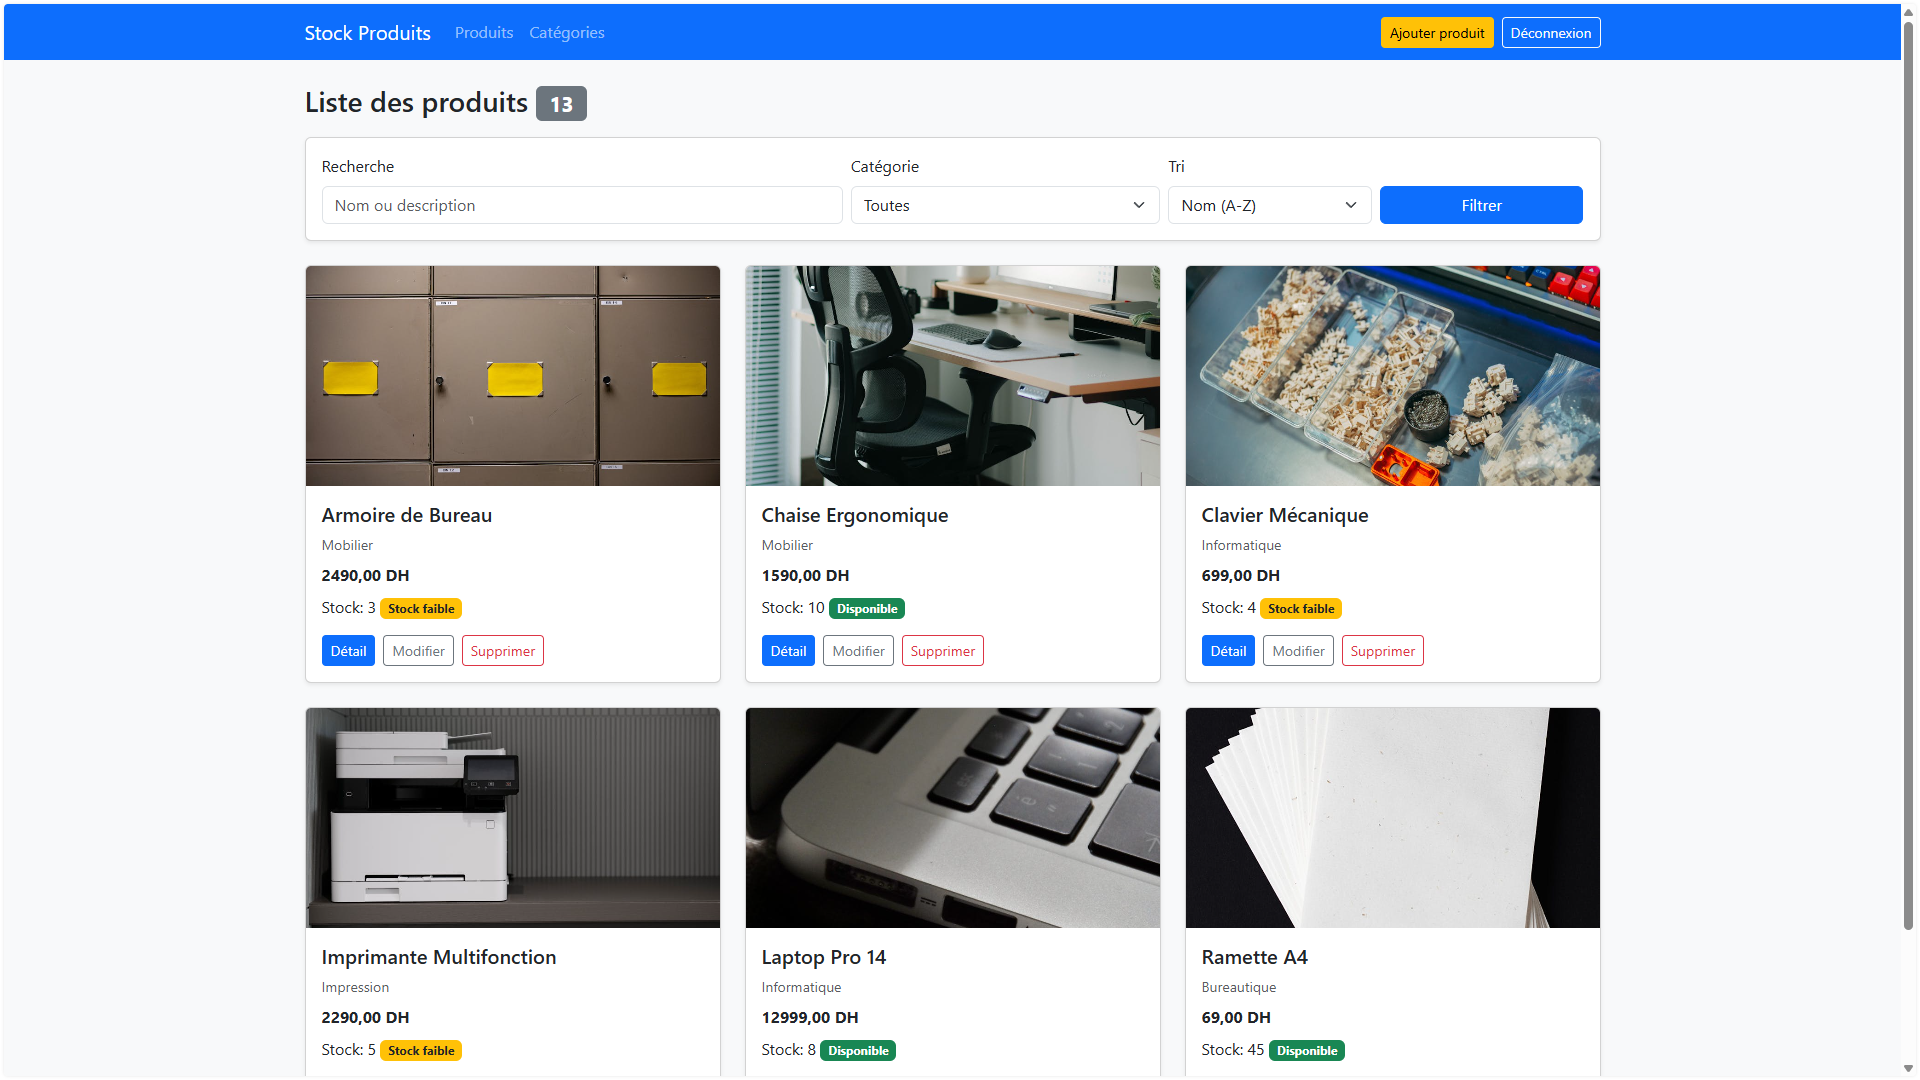
\includegraphics[width=0.97\textwidth]{docs/figures/screenshot_admin.png}
  \caption{Interface administrateur : gestion compl\`ete du catalogue produits}
  \label{fig:vue-admin}
\end{figure}

\Needspace{0.62\textheight}
\subsubsection{Vue utilisateur standard}
La Figure~\ref{fig:vue-user} met en \'evidence la restriction des droits pour le profil \texttt{viewer} : consultation seule, sans op\'erations d'\'edition/suppression.

\begin{figure}[H]
  \centering
  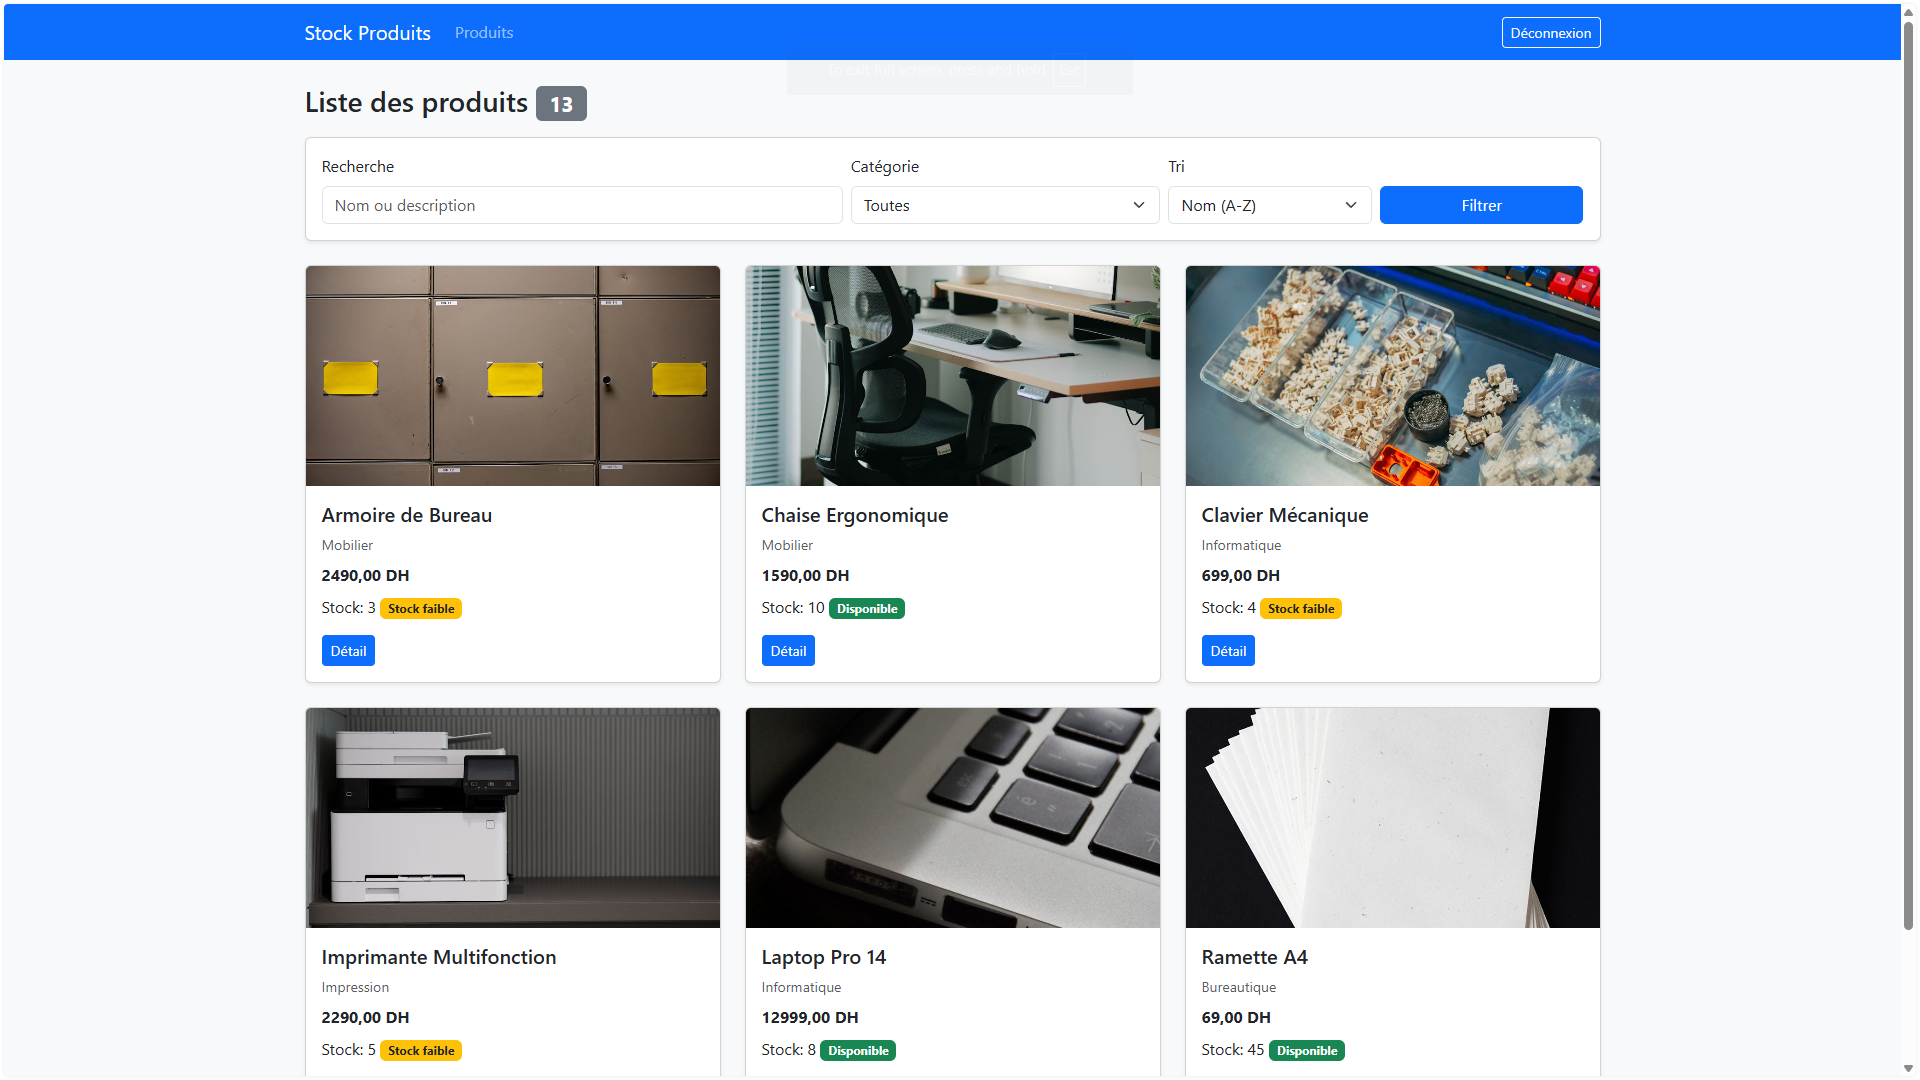
\includegraphics[width=0.97\textwidth]{docs/figures/screenshot_user.png}
  \caption{Interface utilisateur standard : consultation sans droits de gestion}
  \label{fig:vue-user}
\end{figure}

\subsection{Diagrammes UML}
\Needspace{0.80\textheight}
\subsubsection{Diagramme de cas d'utilisation}
\textbf{Fichier source docs :} \texttt{docs/diagrames UML/Diagramme de cas d'utilisation.svg}

Ce diagramme (Figure~\ref{fig:uml-use-case}) formalise les interactions entre acteurs et fonctionnalit\'es du syst\`eme. Il joue un r\^ole de cadrage fonctionnel en visualisant la couverture des besoins par profil. Son interpr\'etation confirme que la plateforme distingue clairement les capacit\'es de consultation et de gestion.

\begin{figure}[H]
  \centering
  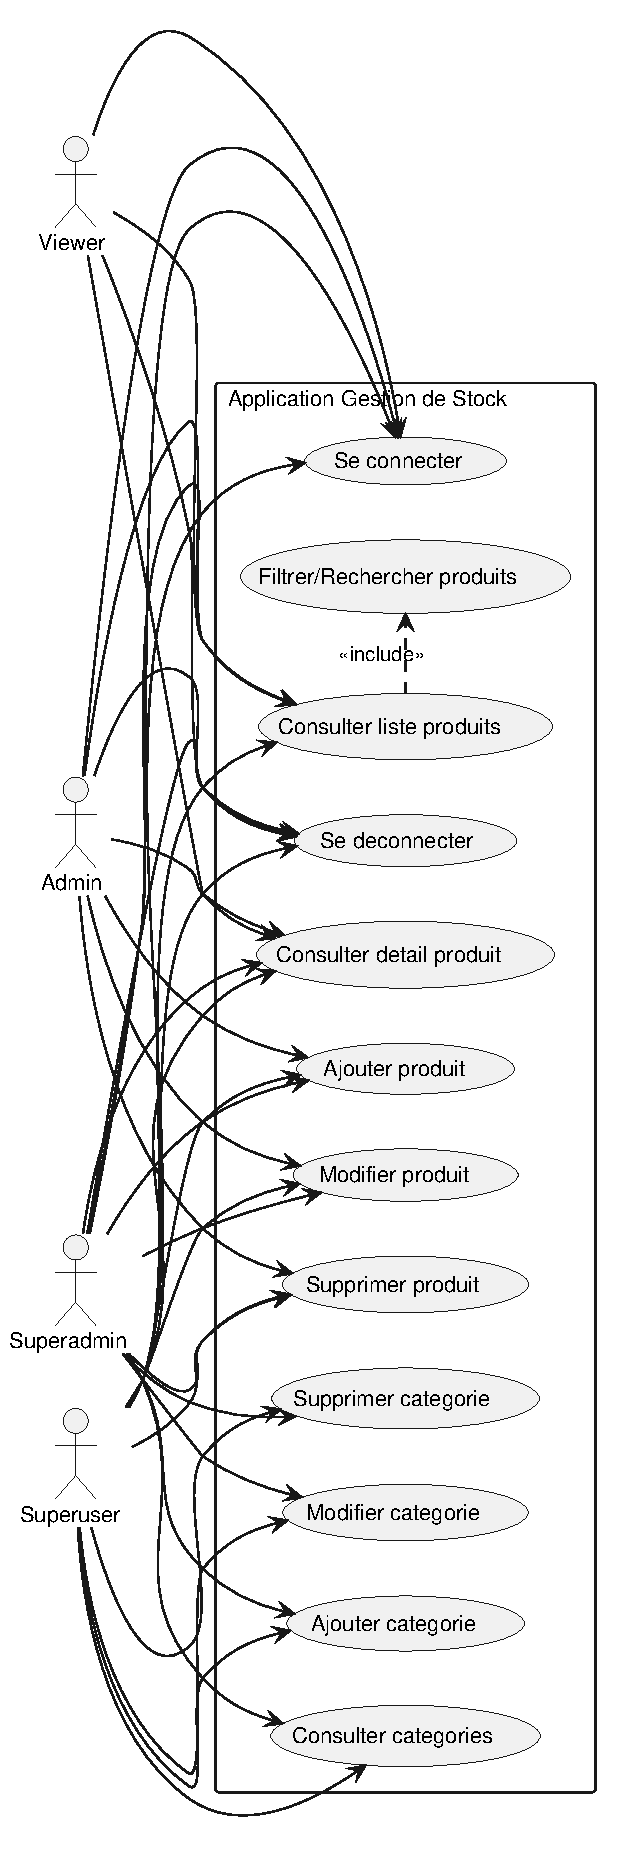
\includegraphics[width=0.50\textwidth,height=0.56\textheight,keepaspectratio]{docs/figures/uml_use_case.pdf}
  \caption{Diagramme UML de cas d'utilisation}
  \label{fig:uml-use-case}
\end{figure}

\Needspace{0.72\textheight}
\subsubsection{Diagramme de classes}
\textbf{Fichier source docs :} \texttt{docs/diagrames UML/Diagramme de classes.svg}

Le diagramme de classes (Figure~\ref{fig:uml-class}) repr\'esente la structure statique : entit\'es \texttt{Category} et \texttt{Product}, relation \`a cardinalit\'e 1--N, et \'el\'ements de couche formulaire/contr\^ole. Il sert \`a v\'erifier la coh\'erence de mod\'elisation et l'alignement avec l'impl\'ementation Django.

\begin{figure}[H]
  \centering
  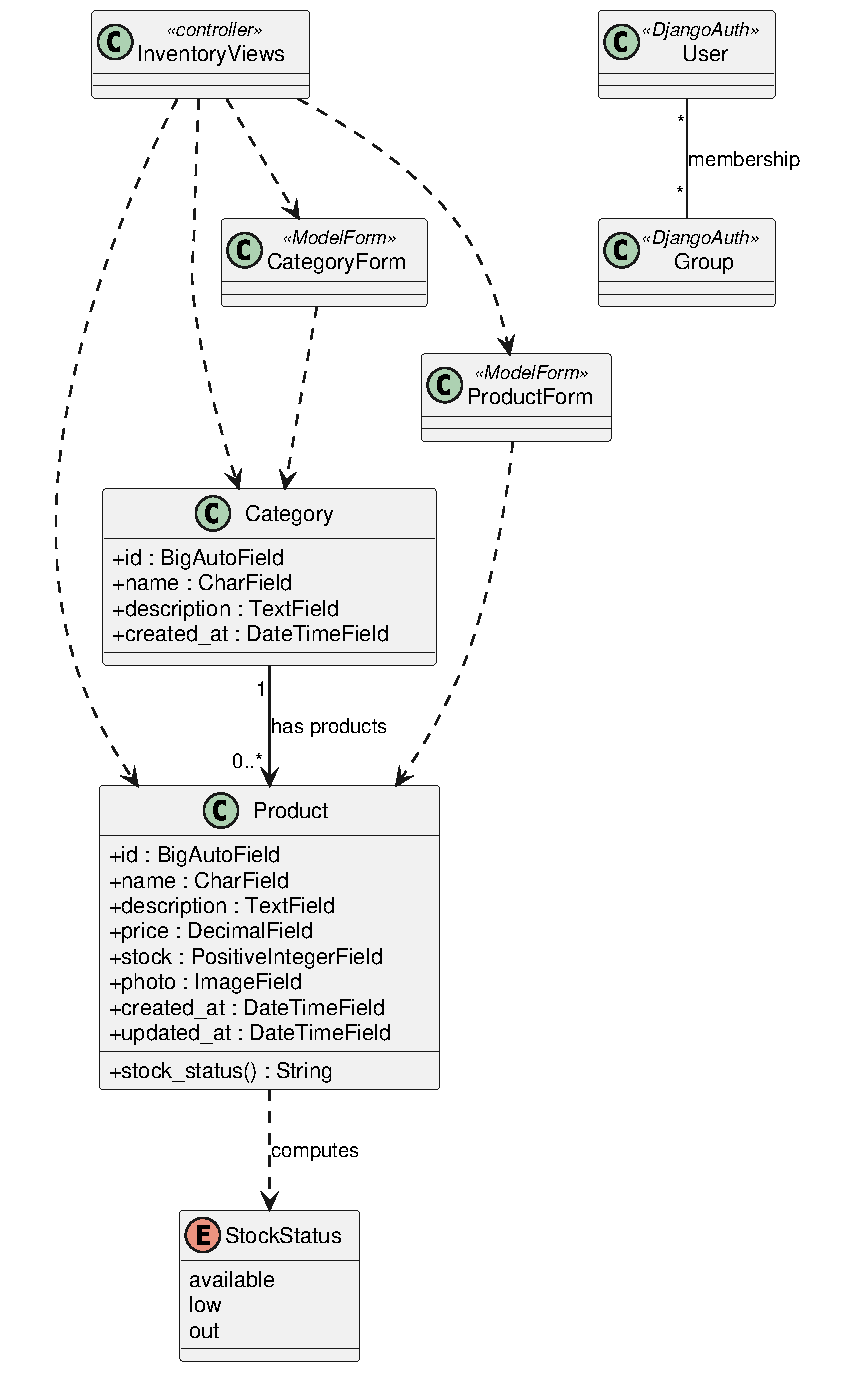
\includegraphics[width=0.78\textwidth,height=0.56\textheight,keepaspectratio]{docs/figures/uml_class_diagram.pdf}
  \caption{Diagramme UML de classes}
  \label{fig:uml-class}
\end{figure}

\Needspace{0.72\textheight}
\subsubsection{Diagramme de composants}
\textbf{Fichier source docs :} \texttt{docs/diagrames UML/Diagramme de composants (07\_component\_diagram.puml).svg}

Le diagramme de composants (Figure~\ref{fig:uml-component}) explicite l'architecture en couches : navigateur, routage, vues, formulaires, mod\`eles, templates, base de donn\'ees et r\'epertoire m\'edia. Il relie directement la conception globale au d\'ecoupage r\'eel du d\'ep\^ot.

\begin{figure}[H]
  \centering
  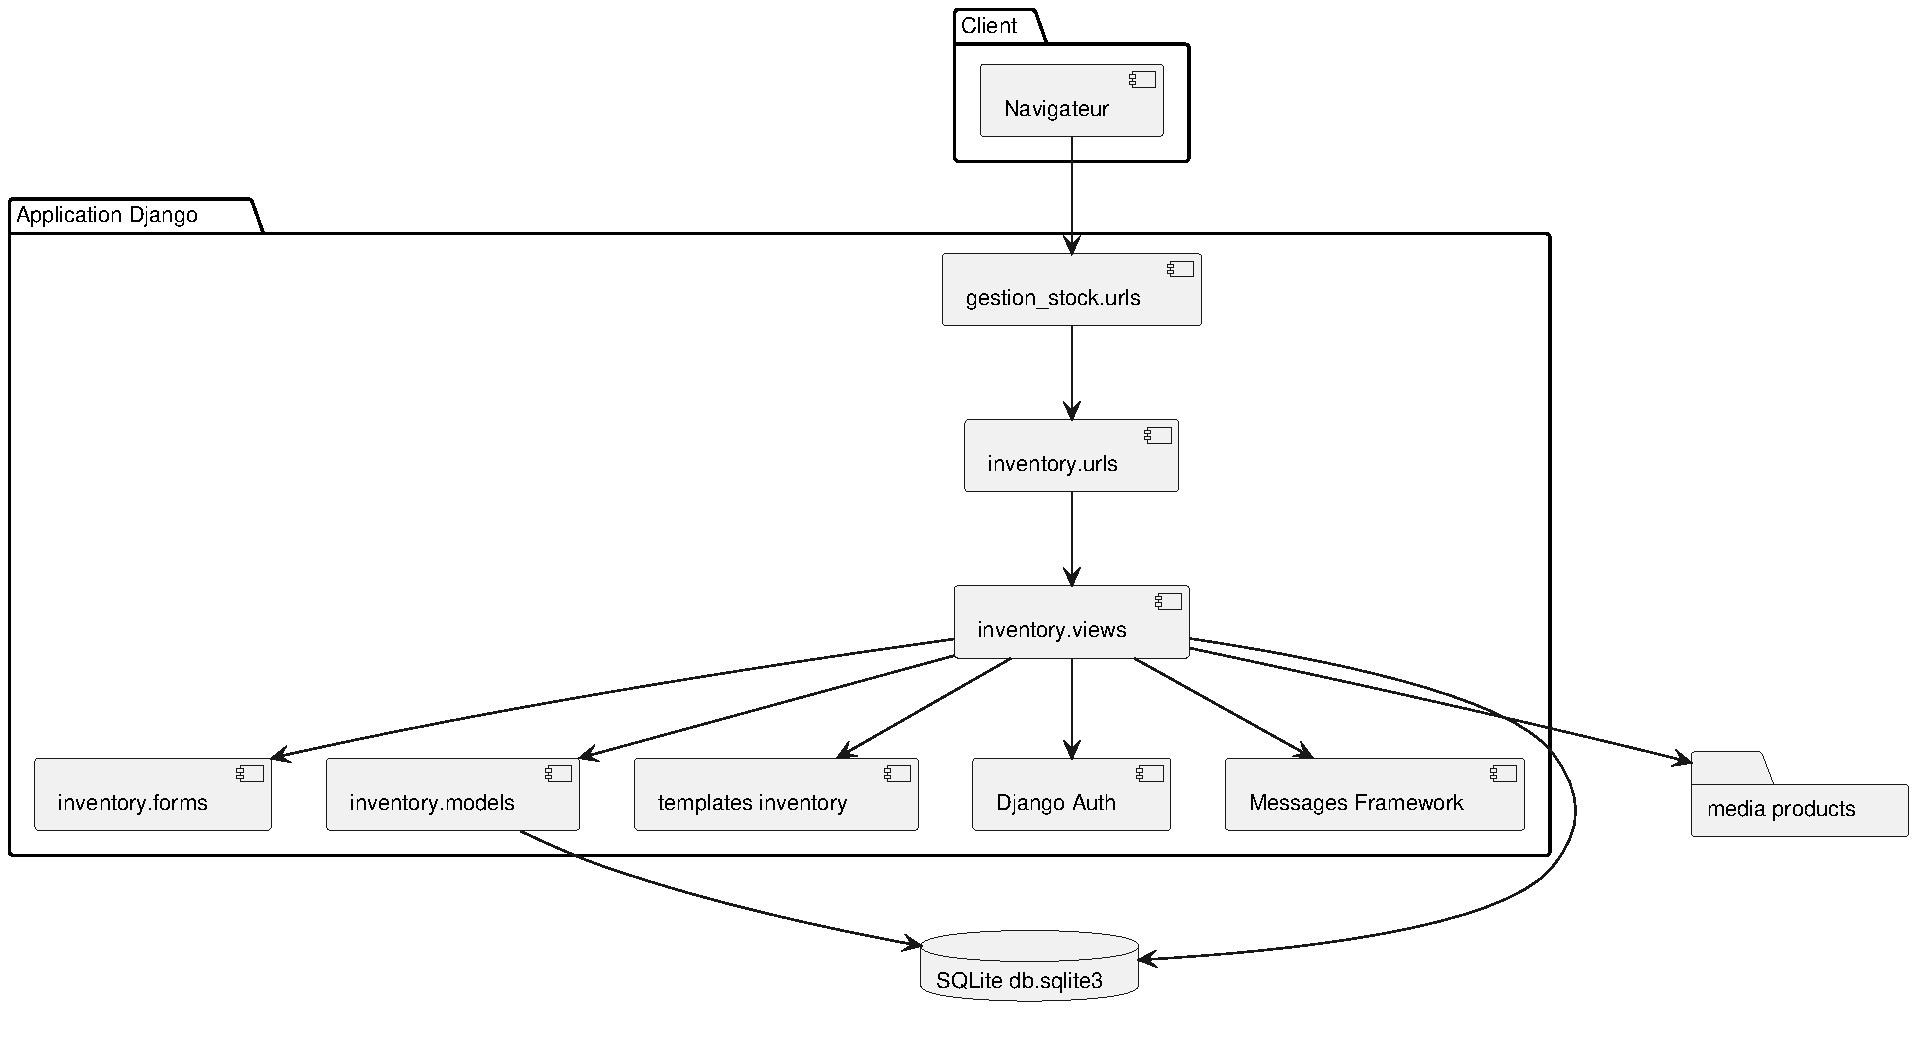
\includegraphics[width=0.94\textwidth,height=0.56\textheight,keepaspectratio]{docs/figures/uml_component_diagram.pdf}
  \caption{Diagramme UML de composants}
  \label{fig:uml-component}
\end{figure}

\Needspace{0.72\textheight}
\subsubsection{Diagramme de s\'equence : consultation de la liste produits}
\textbf{Fichier source docs :} \texttt{docs/diagrames UML/Diagramme de sequence consultation liste produits.svg}

La Figure~\ref{fig:uml-seq-list} d\'etaille la dynamique d'une requ\^ete de consultation : entr\'ee HTTP, traitement des filtres, interrogation SQL et rendu template. Ce diagramme est essentiel pour comprendre la cha\^ine de performance (notamment \texttt{select\_related} et pagination).

\begin{figure}[H]
  \centering
  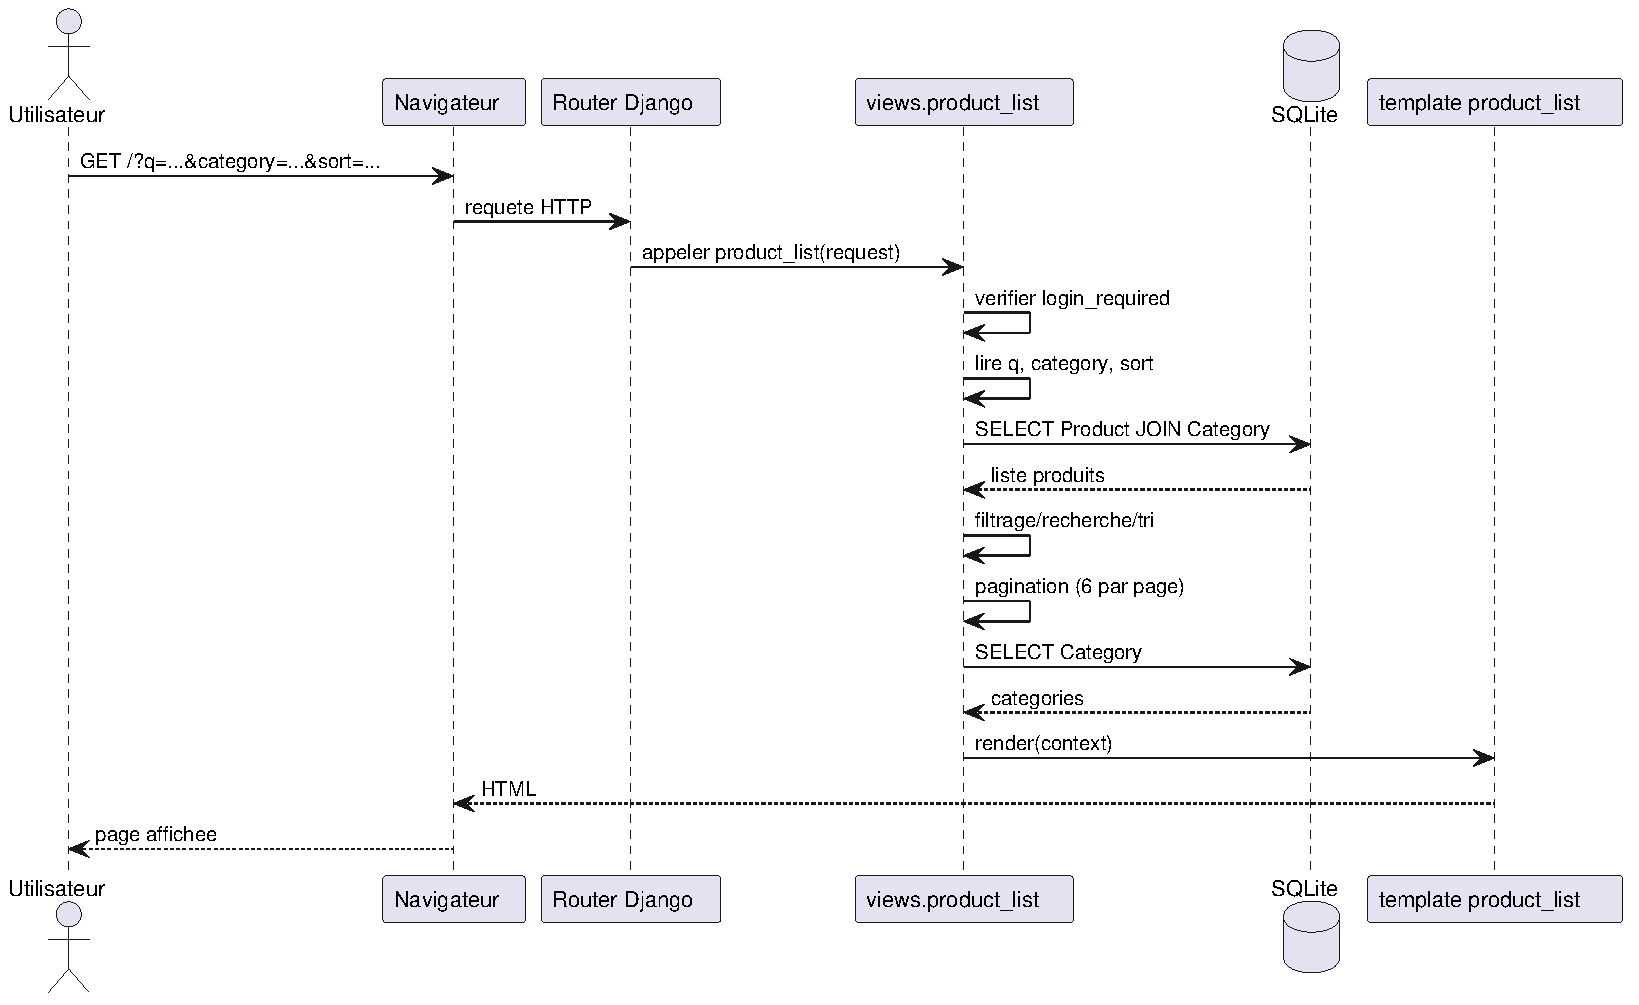
\includegraphics[width=0.94\textwidth,height=0.56\textheight,keepaspectratio]{docs/figures/uml_sequence_product_list.pdf}
  \caption{Diagramme UML de s\'equence - consultation liste produits}
  \label{fig:uml-seq-list}
\end{figure}

\Needspace{0.72\textheight}
\subsubsection{Diagramme de s\'equence : d\'econnexion}
\textbf{Fichier source docs :} \texttt{docs/diagrames UML/Diagramme de sequence deconnexion (04\_sequence\_logout.puml).svg}

Le diagramme de s\'equence de d\'econnexion (Figure~\ref{fig:uml-seq-logout}) d\'ecompose la fermeture de session via POST, l'invalidation de session Django et la redirection vers la page de connexion. Il formalise la correction appliqu\'ee pour \'eliminer les erreurs HTTP 405.

\begin{figure}[H]
  \centering
  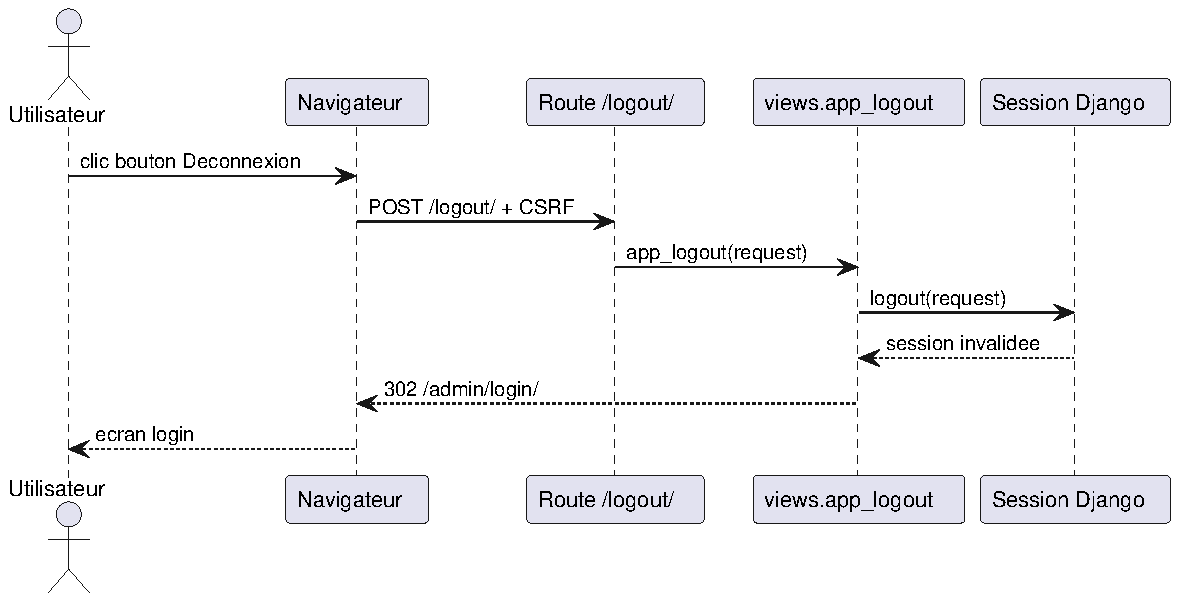
\includegraphics[width=0.84\textwidth,height=0.56\textheight,keepaspectratio]{docs/figures/uml_sequence_logout.pdf}
  \caption{Diagramme UML de s\'equence - d\'econnexion}
  \label{fig:uml-seq-logout}
\end{figure}

\Needspace{0.72\textheight}
\subsubsection{Diagramme d'activit\'e : ajout produit}
\textbf{Fichier source docs :} \texttt{docs/diagrames UML/Diagramme d’activite ajout produit (05\_activity\_add\_product.puml).svg}

La Figure~\ref{fig:uml-activity-add} mod\'elise le flux de cr\'eation d'un produit avec points de d\'ecision : authentification, autorisation, validation formulaire, persistance et retour utilisateur. Ce diagramme relie la logique m\'etier aux contraintes de s\'ecurit\'e.

\begin{figure}[H]
  \centering
  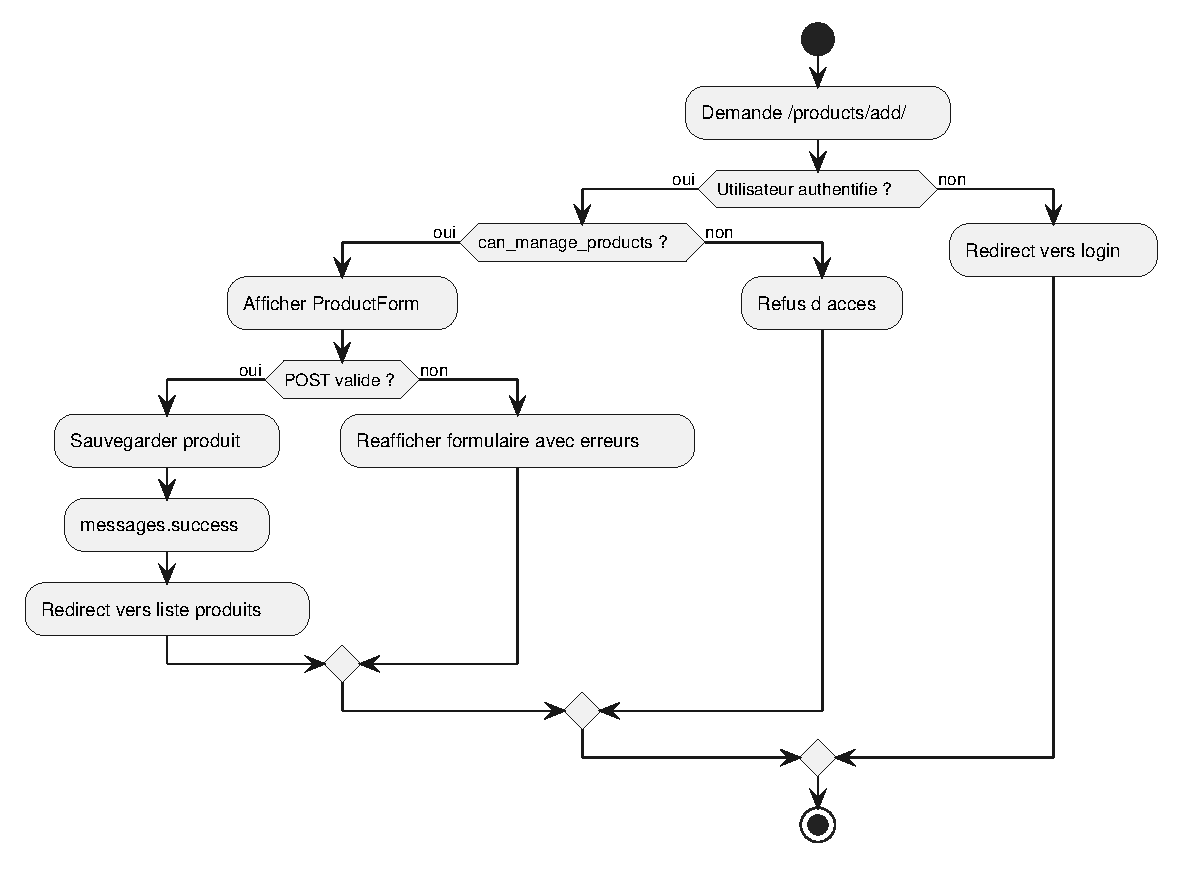
\includegraphics[width=0.86\textwidth,height=0.56\textheight,keepaspectratio]{docs/figures/uml_activity_add_product.pdf}
  \caption{Diagramme UML d'activit\'e - ajout produit}
  \label{fig:uml-activity-add}
\end{figure}

\Needspace{0.72\textheight}
\subsubsection{Diagramme d'\'etats : statut de stock}
\textbf{Fichier source docs :} \texttt{docs/diagrames UML/Diagramme d'etats corrigé (stock\_status).svg}

Le diagramme d'\'etats (Figure~\ref{fig:uml-state-stock}) repr\'esente les transitions \texttt{available}, \texttt{low}, \texttt{out} selon la quantit\'e. Il ancre visuellement la r\`egle de gestion impl\'ement\'ee dans la propri\'et\'e \texttt{stock\_status} du mod\`ele \texttt{Product}.

\begin{figure}[H]
  \centering
  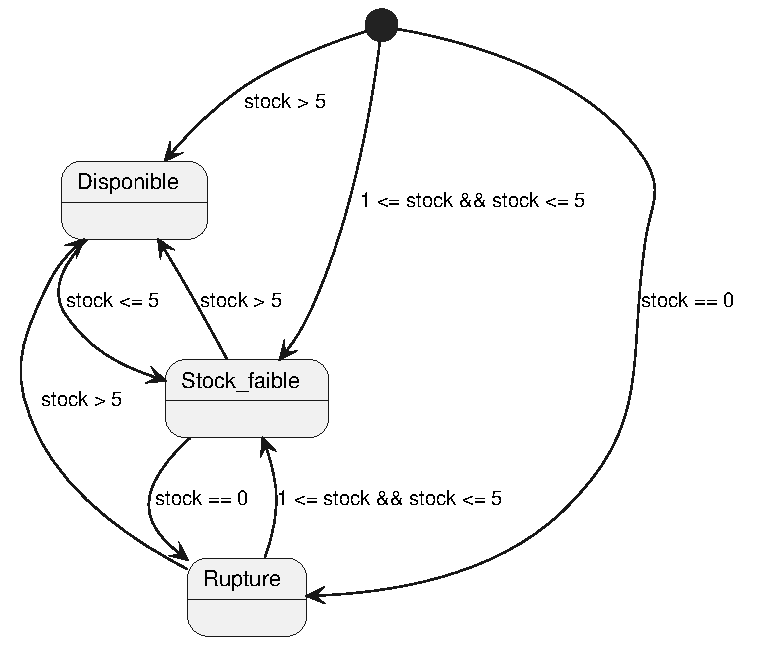
\includegraphics[width=0.68\textwidth,height=0.56\textheight,keepaspectratio]{docs/figures/uml_state_stock_status.pdf}
  \caption{Diagramme UML d'\'etats - statut de stock}
  \label{fig:uml-state-stock}
\end{figure}

\section{Conclusion et perspectives}
Le projet aboutit \`a une application de gestion de stock op\'erationnelle, structur\'ee et adapt\'ee \`a un usage de d\'emonstration ou de prototypage avanc\'e. Les objectifs fonctionnels sont couverts : gestion du catalogue, filtrage, tri, pagination, r\^oles et visualisation de l'\'etat de stock.

Sur le plan technique, le code est lisible, segment\'e et extensible. L'int\'egration de donn\'ees de d\'emonstration, de ressources visuelles et de diagrammes UML renforce la qualit\'e documentaire du projet.

\textbf{Perspectives d'\'evolution :}
\begin{itemize}[leftmargin=1.2cm]
  \item ajout de tests unitaires et d'int\'egration automatis\'es ;
  \item migration vers PostgreSQL pour la production ;
  \item historisation des mouvements de stock (entr\'ees/sorties) ;
  \item ajout d'un tableau de bord analytique (statistiques, alertes) ;
  \item mise en place d'une API REST (Django REST Framework) pour int\'egration externe.
\end{itemize}

\end{document}
